\section{Задание 3.}

\textbf{Условие.}

Найдите сумму числового ряда с помощью разложения функции $f(x)$ в ряд Фурье по косинусам

\begin{gather*}
    \sum_{n = 1}^\infty \frac{1}{(2n - 1)^2} \\
    f(x) = x, x \in (0, \pi)
\end{gather*}

\vspace{10mm}

\textbf{Решение.}

Чтобы разложить функцию по косинусам отразим функцию относительно $0y$ и получим следующее:\\

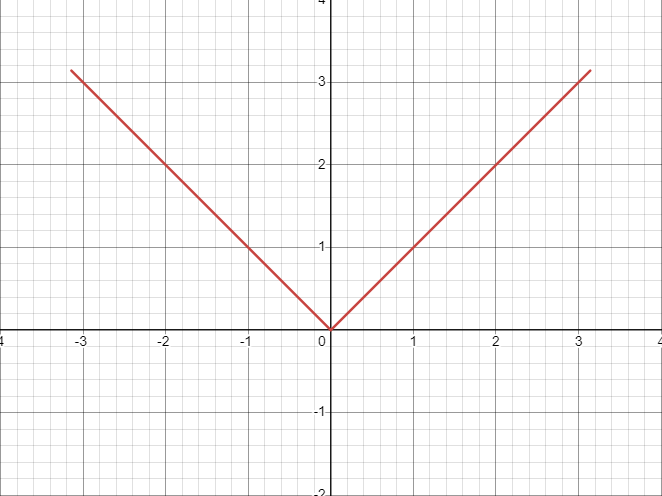
\includegraphics[width=10cm]{images/3-01}

$b_n$ будет 0, ведь функция четная. Тогда найдем свободный член и $a_n$.

{$\displaystyle a_0 = \frac{1}{\pi}\int\limits_{-\pi}^{\pi} f(x) dx = \frac{2}{\pi}\int\limits_{0}^{\pi} x dx =
\frac{x^2}{\pi}\Big|_{0}^{\pi} = \pi$}

{$\displaystyle a_n = \frac{1}{\pi}\int\limits_{-\pi}^{\pi}x \cos(nx)dx = \frac{2}{\pi}\int\limits_{0}^{\pi}x \cos(nx)dx =
\frac{2}{n\pi}\bigl( x\sin(nx) \Big|_{0}^{\pi}- \int\limits_{0}^{\pi}\sin(nx)dx\bigr) =
\frac{2}{n\pi}\bigl(\pi\sin(\pi n) + \frac{1}{n}\cos( nx)\Big|_{0}^{\pi}\bigr) =
\frac{2}{n\pi}\bigl(\pi\sin(\pi n) + \frac{1}{n}\cos(\pi n) - \frac{1}{n}) =
\frac{2(\pi n \sin(n\pi) + \cos(n\pi) - 1)}{\pi n^2}$}\\

$\forall n: \ \sin(\pi n) = 0$

Тогда {$\displaystyle y(x) = \frac{\pi}{2} + 2\sum\limits_{n = 1}^{\infty}\frac{2}{n^2\pi}\bigl(\cos(\pi n) - 1) \cos(nx)$}

Заметим, что $n \divby 2: \cos(n \pi) - 1 = 0, n \not\divby 2: \cos(n \pi) - 1 = -2 \Rightarrow $ в ряду будут только нечетные члены, то есть:
    {$\displaystyle y(x) = \frac{\pi}{2} - 4\sum\limits_{n = 1}^{\infty}\frac{1}{(2n - 1)^2 \pi}\cos((2n-1)x)
= x$}

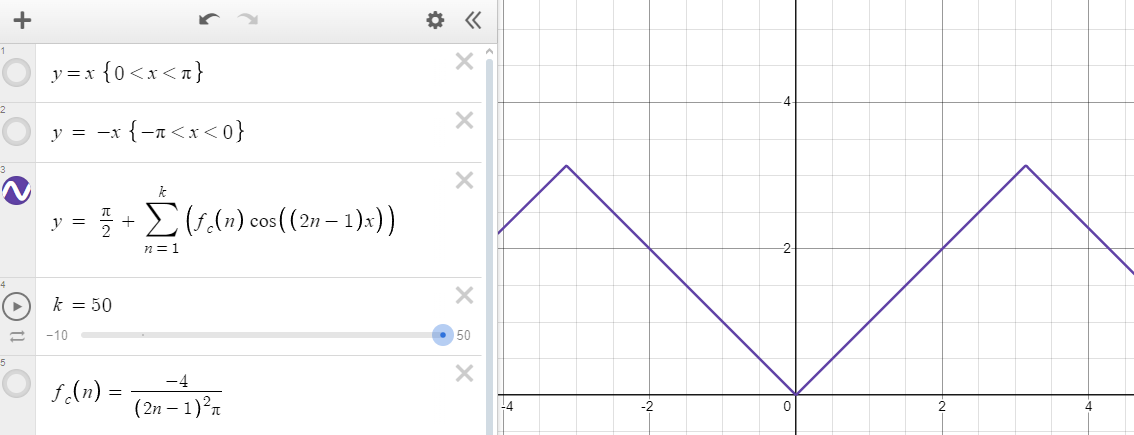
\includegraphics[width=13cm]{images/3-02}

Давайте теперь выразим {$\displaystyle \sum\limits_{n=1}^{\infty}\frac{1}{(2n-1)^2}$} из полученного ряда:\\
    {$\displaystyle y(0) = \frac{\pi}{2} - 4 \sum\limits_{n = 1}^{\infty} \frac{1}{(2n-1)^2 \pi} =
    \frac{\pi}{2} - \frac{4}{\pi} \sum\limits_{n = 1}^{\infty} \frac{1}{(2n-1)^2} = 0 \Rightarrow
    \sum\limits_{n = 1}^{\infty} \frac{1}{(2n-1)^2} = \frac{\pi}{2} \cdot \frac{\pi}{4} = \frac{\pi^2}{8} \approx 1.23$}

\textit{Ответ}: {$\displaystyle \sum\limits_{n = 1}^{\infty} \frac{1}{(2n-1)^2 \pi} = \frac{\pi^2}{8} \approx 1.23$}

\clearpage
